\documentclass[letterpaper, 10 pt, conference]{ieeeconf}
\IEEEoverridecommandlockouts                              % This command is only
                                                          % needed if you want to

                                                          % use the \thanks command
\overrideIEEEmargins
%% \usepackage[dvips]{graphicx}
\usepackage{graphicx}
\usepackage{times}

% numbers option provides compact numerical references in the text. 
\usepackage{multicol}
\usepackage{times}
\usepackage{cite}
\usepackage{algorithm}
\usepackage{algorithmic}
\usepackage{array}

\newcommand{\vecmat}[1]{\mbox{\boldmath \(#1\)}}
%\renewcommand{\labelenumi}{(\arabic{enumi})}
%\renewcommand{\labelfigure}{Fig.figure}

%\newcommand{\matsize}[2]{\in\vecmat{R}^{#1\times #2}}
\newcommand{\matsize}[2]{\in\Re^{#1\times #2}}

%\newcommand{\vecsize}[1]{\in \vecmat{R}^{#1}}
\newcommand{\vecsize}[1]{\in \Re^{#1}}

\newcommand{\hinf}{\(H_{\infty}\)}

\newcommand{\define}{\stackrel{\triangle}{=}}

\newcommand{\eqref}[1]{Eq.(\ref{#1})}

\newcommand{\figref}[1]{Fig.~\ref{#1}}

\newcommand{\tabref}[1]{Table~\ref{#1}}

\newcommand{\argmin}{\mathop{\rm argmin}\limits}
\newcommand{\argmax}{\mathop{\rm argmax}\limits}


% \pdfinfo{
%    /Author (Homer Simpson)
%    /Title  (Robots: Our new overlords)
%    /CreationDate (D:20101201120000)
%    /Subject (Robots)
%    /Keywords (Robots;Overlords)
% }

% paper title
\title{\bf Reducing Hardware Experiments for Model Learning and \\Policy
Optimization}

% You will get a Paper-ID when submitting a pdf file to the conference system
\author{Sehoon Ha$^1$ and Katsu Yamane$^2$%
\thanks{$^1$Sehoon Ha is with Georgia Institute of Technology.  He was
at Disney Research, Pittsburgh when this research was conducted.
$^2$K. Yamane is with Disney Research, Pittsburgh.
{\tt\small kyamane@disneyresearch.com}}%
}

\begin{document}

% avoiding spaces at the end of the author lines is not a problem with
% conference papers because we don't use \thanks or \IEEEmembership


% for over three affiliations, or if they all won't fit within the width
% of the page, use this alternative format:
% 
%\author{\authorblockN{Michael Shell\authorrefmark{1},
%Homer Simpson\authorrefmark{2},
%James Kirk\authorrefmark{3}, 
%Montgomery Scott\authorrefmark{3} and
%Eldon Tyrell\authorrefmark{4}}
%\authorblockA{\authorrefmark{1}School of Electrical and Computer Engineering\\
%Georgia Institute of Technology,
%Atlanta, Georgia 30332--0250\\ Email: mshell@ece.gatech.edu}
%\authorblockA{\authorrefmark{2}Twentieth Century Fox, Springfield, USA\\
%Email: homer@thesimpsons.com}
%\authorblockA{\authorrefmark{3}Starfleet Academy, San Francisco, California 96678-2391\\
%Telephone: (800) 555--1212, Fax: (888) 555--1212}
%\authorblockA{\authorrefmark{4}Tyrell Inc., 123 Replicant Street, Los Angeles, California 90210--4321}}


\maketitle
\thispagestyle{empty}
\pagestyle{empty}

\begin{abstract}
Conducting hardware experiment is often expensive in various aspects
 such as potential damage to the robot and the number of people required
 to operate the robot safely.
Computer simulation is used in place of hardware in such cases, but it
 suffers from so-called simulation bias in which policies tuned in
 simulation do not work on hardware due to differences in the two systems.
Model-free methods such as Q-Learning, on the other hand, do
 not require a model and therefore can avoid this issue.
However, these methods typically require a large number of experiments,
 which may not be realistic for some tasks such as humanoid
 robot balancing and locomotion.
This paper presents an iterative approach for learning hardware models
 and optimizing policies with as few hardware experiments as
 possible. 
Instead of learning the model from scratch, our method learns the
 difference between a simulation model and hardware.
We then optimize the policy based on the learned model in
 simulation. 
The iterative approach allows us to collect wider range of data for
 model refinement while improving the policy.
\end{abstract}

\newlength{\figw}
\newlength{\figh}
%\IEEEpeerreviewmaketitle

\section{Introduction}

Conducting hardware experiments is a cumbersome task especially with
large, complex and unstable robots such as full-size humanoid robots.
They may require multiple people to operate to ensure safety of both
operators and the robot; control failures can cause major damage; and even
a minor damage is difficult to troubleshoot due to complexity.

For this reason, simulation is often used to replace hardware
experiments. 
Unfortunately, it is difficult to obtain accurate simulation
models, and therefore it suffers from so-called simulation bias~\cite{bib-kober-survey} in which 
policies tuned in simulation cannot realize the same task with the
hardware system due to differences in the two systems.

This paper presents an iterative approach for model learning and
policy optimization using as few experiments as possible.
Instead of learning the hardware model from scratch, our method reduces
the number of experiments by only learning the difference from a
simulation model.
The policy is then optimized through simulations using the learned
model.
We repeat this process iteratively so that we can refine the model
because the improved policy is more likely to realize wider range of
motions.

The assumption is that three things are essential to policy learning for
complex robots:
\begin{itemize}
\item Learning only the difference from a model is essential to reduce
the number of hardware experiments.  The model can also be used 
	  for optimizing the initial policy.
\item Iterative process is important for inherently unstable robots because
	  we cannot collect enough data using a policy trained only in simulation.
\item The learned model should be stocastic so that it can model
	  sensor and actuator noises.
\end{itemize}

Our target task in this paper is balancing of bipedal robot on a
bongoboard.
To prove the concept, and to better control the noise conditions, we shall use
two simulation models instead of a simulation model and a hardware system.
One of the models is derived by Lagrangian dynamics assuming perfect
contact conditions, while the other model is based on a 2D physics
simulation engine with a more realistic contact model.
These models are different enough that a policy optimized
for the former cannot stabilize the latter.

The rest of the paper is organized as follows.
In Section~\ref{sec:learning_related}, we first review the related work in
machine learning literature in the context of robot control.
Section~\ref{sec:learning_overview} gives an overview of our framework, followed
by more details on the model learning in
Section~\ref{sec:learning_model-learning} and policy optimization in
Section~\ref{sec:learning_policy-optim}.
Section~\ref{sec:learning_results} presents simulation results and analysis.
We finally conclude the paper in Section~\ref{sec:learning_conclusion}.

%%%%%%%%%%%%%%%%%%%%%%%%%%%%%%%%%%%%%%%%%%%%%%%%%%%%%%%%%%%%%
\section{Related Work} \label{sec:learning_related}

Difference between a robot and its simulation model becomes a serious
problem when we try to use controllers obtained by model-based
optimization or tuned in simulation.
Classical parameter identification
techniques~\cite{bib-khalil-identification} partially solve this
problem by fitting model parameters to experimental data, but they
are still limited to factors that can actually be modeled. 
Furthermore, these approaches assume that the data set is large enough
to accurately estimate the parameters.
In large and unstable systems such as humanoid robots, it is often
difficult to collect enough data~\cite{bib-humanoids2011-calibration}.

Another approach is model-free policy optimization, where the policy is
improved through a number of hardware trials~\cite{bib-morimoto-standup,bib-kober-primitives}.
Unfortunately, these methods generally require hundreds of
trials, which is unrealistic for tasks such as humanoid balancing and
locomotion.
One way to overcome this issue is to limit the parameter space by using
task-specific primitives~\cite{bib-nakanishi-adaptation} or to provide a
good initial trajectory by human
demonstration~\cite{bib-atkeson-demonstration}.
However, it is not clear how to extend these approaches to dynamically
unstable robots or tasks that cannot described by joint trajectories.

A number of researchers have attempted to overcome the drawbacks of
these approaches by combining simulation and real-world data~\cite{bib-sutton-integrated,bib-moore-prioritized-sweeping,bib-peng-incremental}.
Abbeel et al.~\cite{bib-abbeel-inaccurate} used an inaccurate model to
estimate the derivative of the cost with respect to the policy
parameters.
Ko et al.~\cite{bib-ko-blimp} used Gaussian Process to model the
difference between a nonlinear dynamics model and the actual dynamics
and applied the model to reinforcement learning for yaw control of a
blimp.  However, they do not iterate the process to refine the model.
Deisenroth et al.~\cite{bib-deisenroth-data-efficient} also used
Gaussian Process for learning the dynamics model from scratch.
Ross and Bagnell~\cite{bib-ross-agnostic} theoretically proved that
their iterative system identification method converges even the system
is not in the assumed class.
Please refer to Section 6 of~\cite{bib-kober-survey} for more complete
survey on this topic.

%%%%%%%%%%%%%%%%%%%%%%%%%%%%%%%%%%%%%%%%%%%%%%%%%%%%%%%%%%%%%
\section{Overview} \label{sec:learning_overview}

We developed an iterative reinforcement learning process to alternatley
refine the model and policy.
Figure~\ref{fig:learning_framework} illustrates the approach.

\begin{figure}[tb]
\begin{center}
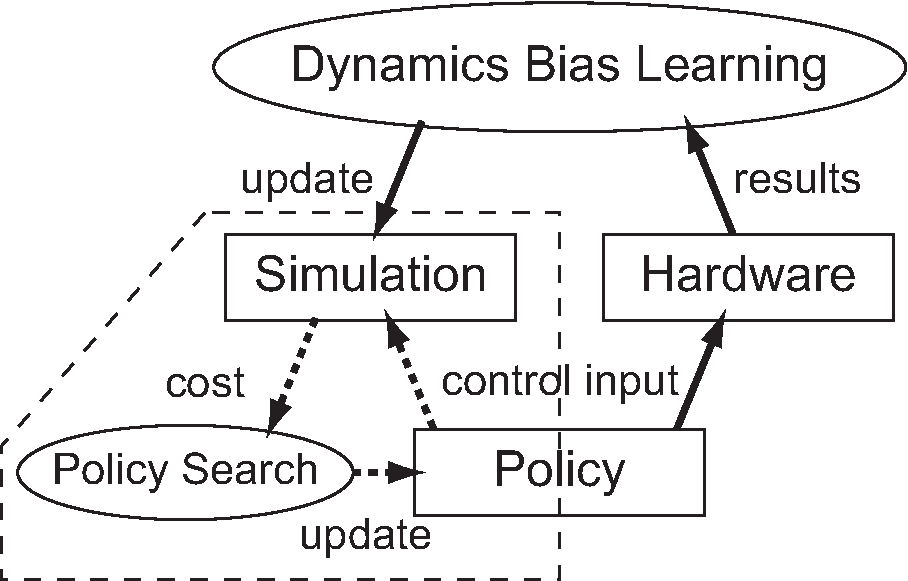
\includegraphics[width=60mm]{eps/framework.pdf}
\caption{Framework of our approach.}
\label{fig:learning_framework}
\end{center}
\end{figure}

The three main components are simulation, hardware, and policy.
{\em Simulation} is based on a model of the robot hardware, and cheap to run.
{\em Hardware} is the real robot and therefore more expensive to run.
Both simulation model and robot hardware are controlled by control
inputs computed by the {\em policy}.

The framework includes two iteration loops that run with different
cycles. 
The outer loop (solid arrows) is the {\em dynamics bias learning}
process that uses the experimental data from hardware to train the
simulation model. 
The inner loop (dashed arrows) is the {\em policy search} process that
uses the simulation model to optimize the policy based on a given cost
function.

Our framework adapts some of the ideas used in prior work.
Similarly to~\cite{bib-ko-blimp}, we use Gaussian Process to model the
difference between a dynamics model and actual robot dynamics.
On the other hand, we also adopt the iterative learning scheme as
in~\cite{bib-abbeel-inaccurate} because the performance of the initial
controller is usually not good enough to learn accurate dynamics model.
We also chose to directly optimize the policy parameters instead of
learning the value function, as in~\cite{bib-deisenroth-data-efficient}.

We compare our framework with conventional direct policy search
represented in \figref{learning_fig:direct-policy-search}.
This approach only has the policy search loop that uses the hardware
directly to obtain the control cost for policy search.
It usually requires a large number of hardware trials, which
is unrealistic for our target robots and tasks.

\begin{figure}[tb]
\begin{center}
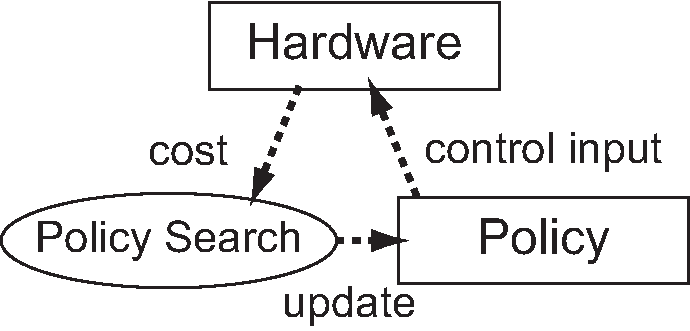
\includegraphics[width=40mm]{eps/direct_policy_search.pdf}
\caption{Direct policy search.}
\label{fig:learning_direct-policy-search}
\end{center}
\end{figure}

The goal of this work is to reduce the number of dynamics bias
learning loops that involve hardware experiments.
On the other hand, we can easily run many policy search loops because
we only have to run simulations.


%%%%%%%%%%%%%%%%%%%%%%%%%%%%%%%%%%%%%%%%%%%%%%%%%%%%%%%%%%%%%
\section{Learning the Dynamics Model} \label{sec:learning_model-learning}

\subsection{Dynamics Bias Formulation}

A general form of dynamics of a system with $n$ states and $m$ inputs
can be written as 
\begin{equation}
\vecmat{x}_t = \vecmat{x}_{t-1} + \vecmat{f}\left(\vecmat{x}_{t-1},
\vecmat{u}_{t-1}\right)
\end{equation}
where
\begin{eqnarray*}
\vecmat{x}\vecsize{n} &: & \mbox{robot state}\\
\vecmat{u}\vecsize{m} &: & \mbox{input}\\
\vecmat{f}\colon \Re^{n}\times\Re^{m}\rightarrow \Re^{n} &: & \mbox{system dynamics function}.
\end{eqnarray*}

The goal of learning is to obtain $\vecmat{f}$ such
that the model can accurately predict the system's behavior.
In this paper, we employ one of the non-parametric models, Gaussian
Process (GP) model.
Learning $\vecmat{f}$ without prior knowledge, however, is expected to
require a large amount of data to accurately model the system dynamics.

For many robots, we can obtain an approximate dynamics model by using,
for example, Lagrangian dynamics.
We denote such model by $\vecmat{f}'$.
Instead of learning $\vecmat{f}$ that requires a large amount of data,
our idea is to learn the difference between $\vecmat{f}'$ and the real
dynamics:
\begin{equation}
\vecmat{x}_t = \vecmat{x}_{t-1} + \vecmat{f}'\left(\vecmat{x}_{t-1},
\vecmat{u}_{t-1}\right) +
\vecmat{g}_D\left(\vecmat{x}_{t-1},\vecmat{u}_{t-1}\right)
\end{equation}
where $\vecmat{g}_D\colon
\Re^{n}\times\Re^{m}\rightarrow\Re^{n}$ is the difference
model to be learned and $D$ 
represents the set of data used for learning the model.
In this paper, we call $\vecmat{g}_D$ as dynamics bias.

Our expectation is that $\vecmat{f}'$ is a good approximation of the system
dynamics, and therefore learning $\vecmat{g}_D$ requires far smaller
data set than learning $\vecmat{f}$ from scratch.

\subsection{Gaussian Process}

% general review of GP

Gaussian Process (GP)~\cite{bib-rasmussen-gp} is a stochastic model that
represents the relationship between $r$ inputs
$\tilde{\vecmat{x}}\vecsize{r}$ and a scalar output $y$.
For the covariance function, we use the sum of a squared exponential
and noise functions:
\begin{equation}
k\left(\tilde{\vecmat{x}}, \tilde{\vecmat{x}}'\right) = \alpha^2 \exp \left(
-\frac{1}{2} \left(\tilde{\vecmat{x}} - \tilde{\vecmat{x}}'\right)^T
\vecmat{\Lambda}^{-1} \left(\tilde{\vecmat{x}} - \tilde{\vecmat{x}}'\right)
\right)
+ \delta_{\tilde{\vecmat{x}}, \tilde{\vecmat{x}}'} \sigma^2
\end{equation}
where $\alpha^2$ is the variance of the latent function, $\sigma^2$ is
the noise variance, and $\vecmat{\Lambda}^{-1}$ is a positive-definite
matrix. 
Assuming that $\vecmat{\Lambda}^{-1}$ is a diagonal matrix whose
elements are $\left\{l_1, l_2, \ldots, l_r\right\}$, the set of
parameters $\vecmat{\theta} =
\left(l_1,l_2,\ldots,l_r,\alpha^2,\sigma^2\right)$ is called
hyper-parameters. 

With $N$ pairs of training inputs $\tilde{\vecmat{x}}_i$ and outputs
$y_i$ $(i=1,2,\ldots,N)$, we can predict the output for a new
input $\tilde{\vecmat{x}}^*$ by
\begin{equation}
y^* = \vecmat{k}_*^T \vecmat{K}^{-1} \vecmat{y}
\end{equation}
with variance
\begin{equation}
\sigma^2 = k(\tilde{\vecmat{x}}^*, \tilde{\vecmat{x}}^*) -
\vecmat{k}_*^{T} \vecmat{K}^{-1} \vecmat{k}_*
\end{equation}
where $\vecmat{K} = \left\{ k(\tilde{\vecmat{x}}_i,
\tilde{\vecmat{x}}_j)\right\} \matsize{N}{N}$ and 
$\vecmat{k}_* = \left\{
k\left(\tilde{\vecmat{x}}^*,\tilde{\vecmat{x}}_i\right)\right\} 
\vecsize{N}$.

% In our model, the input to the GP is a tuple of current state and
% torques:
% \begin{equation}
% \tilde{\vecmat{x}}_{t-1} = \left( \vecmat{x}_{t-1}^T\;
% \vecmat{u}_{t-1}^T\right)^T
% \end{equation}
% while the output is the difference from the next state predicted by the
% physical model:
% \begin{equation}
% \vecmat{y}_t = \vecmat{x}_t - \vecmat{x}_{t-1} -
% \vecmat{f}'\left(\vecmat{x}_{t-1}, \vecmat{u}_{t-1}\right)
% \end{equation}


The hyper-parameters are normally optimized to maximize the marginal
likelihood of producing the training data.
In our setting, however, optimizing hyper-parameters often results in
over-fitting due to the small number of training data.
We therefore manually adjust the hyper-parameters by looking at the
policy optimization results.


\subsection{Learning} \label{sec:learning_learning}

We collect the input and output data from hardware experiments to train
the dynamics bias model.
For multiple-output systems, we use one GP for each dimension and train each GP
independently using the outputs obtained from the same set of inputs.

The inputs to the GP models are the current state and input,
$\tilde{\vecmat{x}}_t = \left(\vecmat{x}_{t-1}^T\;
\vecmat{u}_{t-1}^T\right)^T$, while the outputs are the difference
between the measured state and the prediction of the simulation model:
\begin{equation}
\vecmat{\Delta}_t = \vecmat{x}_t - \vecmat{x}_{t-1} - \vecmat{f}'\left(\vecmat{x}_{t-1},\vecmat{u}_{t-1}\right).
\end{equation}
We collect a set of input and output pairs from hardware experiments.

The computational cost for learning increases rapidly as the training
data increases.
We therefore remove some of the samples from learning data set.
First, we downsample the data because similar states do not improve
model accuracy.
We then remove the samples where the robot and board are no longer
balancing on the wheel.
Next, we discard the samples whose states are too far away from the static
equilibrium state or too difficult to recover balance, since designing a
controller in such areas of the state space does not make much sense. 
Finally, we discard the frames that are far from the prediction by the
simulation model in order to remove outliers that may happen due to
sensor erros in hardware experiments.

To summarize, samples with the following properties are not included in
the training data:
\begin{enumerate}
\item The board touches the ground.
\item The board and wheel are detached.
\item The distance from the static equilibrium state is larger than a
	  threshold.
\item The global angle of the robot body exceeds a threshold.
\item The global angle of the board exceeds a threshold.
\item The norm of the velocity exceeds a threshold.
\item The distance from the state predicted by the Lagrangian model is
	  larger than a threshold.
\end{enumerate}


\subsection{Prediction}

In policy search, we use the dynamics bias model to predict the next
state $\vecmat{x}_t$ given the current state $\vecmat{x}_{t-1}$ and input
$\vecmat{u}_{t-1}$.
The GP model predicts the mean
$\bar{\vecmat{\Delta}}_t$ and variance $\vecmat{\sigma}_t$ of the
output, and the mean value is commonly used as the prediction.
A problem with this method is that the prediction is not accurate if the
input is far from any of the training data, especially when the traning
data is sparse as in our case.
Here, we take advantage of the system dynamics model $\vecmat{f}'$ by
weighing the prediction of the GP such that we rely on the model as the
prediction variance becomes larger, i.e.,
\begin{equation}
\vecmat{x}_t = \vecmat{x}_{t-1} + \vecmat{f}'(\vecmat{x}_{t-1}, \vecmat{u}_{t-1}) +
 \exp\left( -d |\vecmat{\sigma}^2|^2\right) \bar{\vecmat{\Delta}}_t
\label{eq:learning_prediction}
\end{equation}
where $d>0$ is a user-defined coefficient.
If $\left(\vecmat{x}_{t-1}^T\;\vecmat{u}_{t-1}^T\right)^T$ is far away
from any learning data, then the last term of \eqref{eq:prediction} is
nearly zero, meaning that we mostly use the prediction by the model.

%%%%%%%%%%%%%%%%%%%%%%%%%%%%%%%%%%%%%%%%%%%%%%%%%%%%%%%%%%%%%
\section{Data-Efficient Reinforcement Learning} \label{sec:learning_policy-optim}

%\subsection{Policy Search}

Algorithm~\ref{alg:learning_learning} summarizes our framework.
The algorithm starts from an empty learning data set $D=\emptyset$ and
the assumption that the simulation model is accurate, i.e.,
$\vecmat{g}=0$.
At each iteration, we first search for an optimal policy using
the simulation model $\vecmat{f}' + \vecmat{g}$.
If the optimal policy does not give satisfactory results with the
simulation model, we clear the model and restart from scratch.
Otherwise, we evaluate the policy by a few hardware experiments to
obtain the maximum cost as well as a new data set $D_i$ for learning.
If the policy successfully achieves the control objective on hardware,
we terminate the iteration.
Otherwise, we append $D_i$ to the existing data set and re-learn the
dynamics bias model $\vecmat{g}$ and repeat the same process until the
maximum number of iterations is reached.

The cost function for policy optimization is
\begin{equation}
Z = c (T-t_{fail}) + \max_{1\leq t \leq T} \vecmat{x}_t^T \vecmat{R}
 \vecmat{x}_t +
\sum_{t=0}^T \vecmat{u}_t^T \vecmat{Q} \vecmat{u}_t
\end{equation}
where $c$ is a user-defined positive constant, $T$ is the number of
simulation frames, $t_{fail}$ is the frame at which the simulation failed, and
$\vecmat{R}\matsize{n}{n},\vecmat{Q}\matsize{m}{m}\geq 0$ are
user-defined weight matrices. 
We set $c = Z_{max}$ to make sure that the cost function value always
exceed $Z_{max}$ if a policy fails to keep the robot balanced for $T$
frames. 
The first term penalizes policies that cannot balance the model for at
least $T$ frames. 
To determine failure, we use the criteria 1)--6) described in
Section~\ref{sec:learning_learning}.
The second term tries to minimze the maximum distance from the
static equilibrium state.
The third term considers the total energy consumption for control.


\begin{algorithm}[t]
\caption{Data-efficient reinforcement learning}
\label{alg:learning_learning}
\begin{algorithmic}[1]
\REQUIRE nominal model $\vecmat{f}$
\STATE initialize $D=\emptyset$ and $\vecmat{g} = 0$ 
\STATE $i \leftarrow 0$
\WHILE{$i < N_{out}$}
\STATE $p \leftarrow$ policy optimized for $\vecmat{g}$
\STATE $Z_g \leftarrow$ evaluate policy $p$ on $\vecmat{g}$
\IF{$Z_g > Z_{max}$}
\STATE initialize the simulation model: $D=\emptyset$ and $\vecmat{g} = 0$
\ENDIF
\STATE $Z_r, D_i \leftarrow$ evaluate $p$ with hardware experiments
\IF{$Z_r < Z_{max}$}
\STATE break
\ENDIF
\STATE $D \leftarrow D \cup D_i$
\STATE $\vecmat{g} \leftarrow \vecmat{g}_D$ 
\STATE $i \leftarrow i+1$
\ENDWHILE
\end{algorithmic}
\end{algorithm}

Any numerical optimization algorithm can be used for optimizing the
policy $p$ using the simulation model.
We have found that the DIRECT algorithm~\cite{bib-jones-direct} works
best for our problem.
Theoretically, the DIRECT algorithm is capable of finding the globally
optimal solution relatively quickly.
We terminate the algorithm when the relative change in the cost function
value in an optimization step is under a threshold $\epsilon$, or the
number of cost function evaluations exceeds a threshold $N_{in}$.
DIRECT also requires the upper and lower bounds for each optimization
parameters.

%%%%%%%%%%%%%%%%%%%%%%%%%%%%%%%%%%%%%%%%%%%%%%%%%%%%%%%%%%%%%
\section{Results}  \label{sec:learning_results}

While the final goal of this work is to optimize a policy for hardware
systems, this paper focuses on proof of concept and uses two different
simulation models in place of a simulation model and hardware.
Using a well-controlled simulation environment also gives us the
opportunity to explore different noise types and levels.

\subsection{Bongoboard Balancing}

The task we consider is balancing on bongoboard of a simple legged
robot shown in \figref{learning_fig:bongoboard}(a).
Specifically, we apply the output-feedback controller developed by
Nagarajan and Yamane~\cite{bib-icra14-universal} and attempt to optimize
the gains through model learning and policy search.
The state of the system is $\vecmat{x} = (\alpha_w\; \alpha_b\;
\theta_1^r\; \dot{\alpha}_w\; \dot{\alpha}_b\; \dot{\theta}_1^r)^T$ (see
\figref{learning_fig:bongoboard}(a)), and the outputs we use for feedback control
are 
$\vecmat{z} = (x_p\; \dot{x}_p\; \theta_1^r\; \dot{\theta}_1^r\; \alpha_f)^T$ as
indicated in \figref{learning_fig:bongoboard}(b).

The system has three degrees of freedom, and the only input is the
ankle torque.
Therefore the number of states is $n = 6$ and the number of inputs to
the model is $m=1$.
Then the number of inputs to the GP becomes $r=n+m=7$.

The output-feedback controller takes the five outputs of the models and
compute the ankle torque by
\begin{equation}
u = \vecmat{H} \vecmat{z}
\end{equation}
where $\vecmat{H} = \left(h_1\; h_2\; \ldots\; h_5\right)$ is the
feedback gain matrix.
The policy search process computes the optimal values for the five
elements of the gain matrix. 
In our implementation, we optimize a different set of parameters
$\hat{\vecmat{h}}$ that are mapped to the elements of $\vecmat{H}$ by 
\begin{equation}
h_i = \left\{ 
\begin{array}{cc}
\exp(\hat{h}_i)-1 & \mbox{if }\hat{h}_i \geq 0 \\
-\exp(-\hat{h}_i)+1 & \mbox{if }\hat{h}_i < 0 \\
\end{array}
\right.
\end{equation}
instead of directly optimizing $h_i$.

As mentioned above, we use two models in this paper, one corresponding
to the {\em simulation} and the other corresponding to the {\em
hardware} blocks for \figref{learning_fig:framework}.

The first model is derived by the Lagrangian dynamics formulation as
described in~\cite{bib-icra14-universal}.  This model assumes perfect
contact condition, i.e. no slip or detachment of contacts between the
floor and wheel, the wheel and board, as well as the board and robot
feet.

\begin{figure}[tb]
\begin{center}
%\includegraphics[width=70mm]{eps/dynamicModel2.pdf}
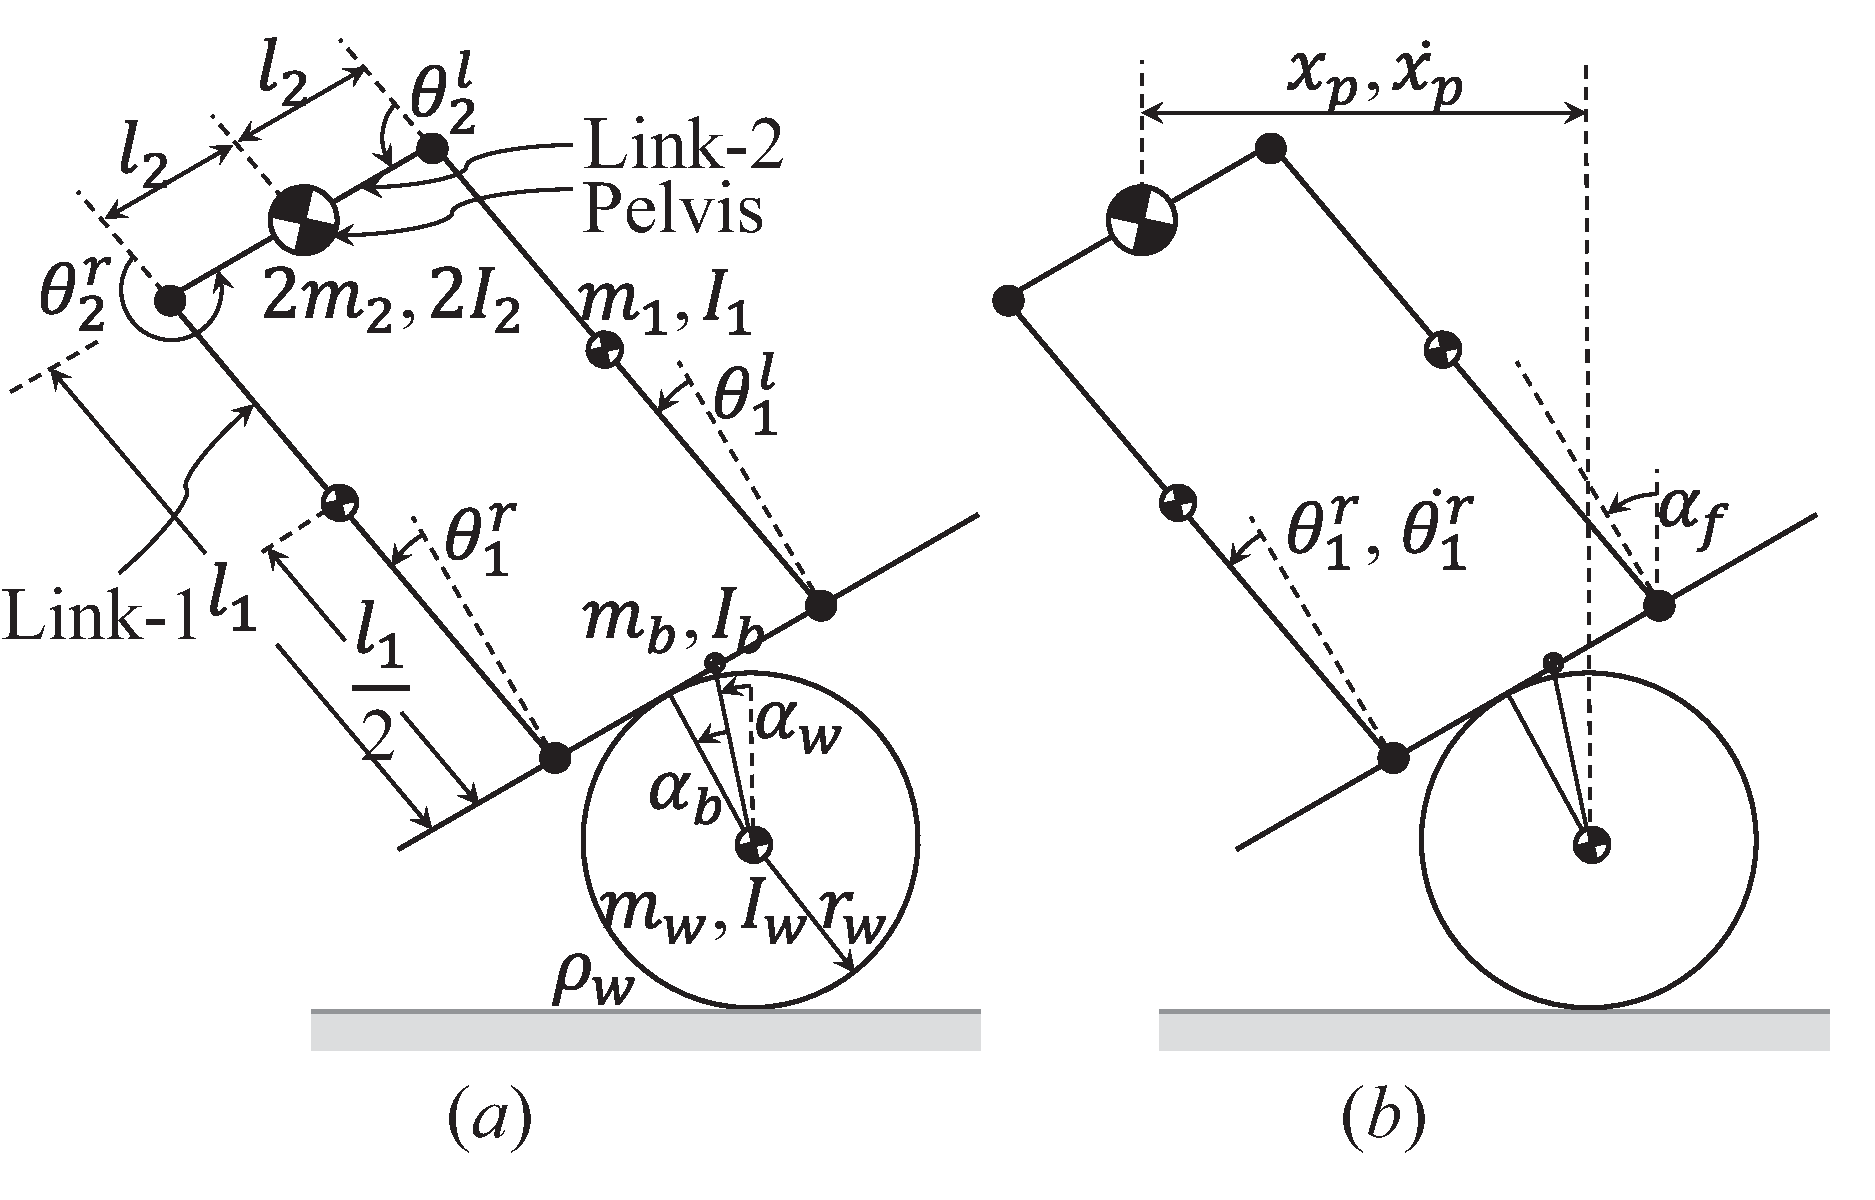
\includegraphics[width=80mm]{eps/dynamicModelNOutputs.pdf}
\caption{Robot balancing on a bongoboard.}
\label{fig:learning_bongoboard}
\end{center}
\end{figure}

% add model equations here

The second model, used in lieu of hardware, is based on a 2D physical
simulation engine called 
Box2D~\cite{bib-box2d}, which uses maximal (Eulerian) coordinate system and
a spring-and-damper contact model. %% correct? 
To make the simulation realistic, we add three types of noise:
\begin{itemize}
\item Torque noise: a zero-mean gaussian noise of variance
	  $\sigma_{\tau}^2$ is added to the robot's ankle joint torque.
\item Joint angle noise: a zero-mean Gaussian noise of variance
	  $\sigma_{p}^2$ is added to the wheel ($\alpha_w$), board
	  ($\alpha_b$), and robot ($\theta_1^r$) angles used for feedback
	  control. 
\item Joint velocity sensor noise: a zero-mean Guassian noise of
	  variance $\sigma_v^2$ is added to the wheel ($\dot{\alpha}_w$),
	  board ($\dot{\alpha}_b$), and robot ($\dot{\theta}_1^r$)
	  anglular velocities.
\end{itemize}
We also randomly choose the initial states in Box2D simulations for
collecting training data for dynamics bias model learning because it is
impossible to set exact initial states in hardware experiments.

Even though both are simulation, the results may be different due to
different contact models and coordinate systems.
In fact, a policy optimized for the Lagrangian model does not always balance
the robot in the second model, which justifies the need for our
framework even in this simple setup.
Figure~\ref{fig:learning_example-math-sim} show an example of using a policy
optmized for the Lagrangian and Box2D models for both the Box2D model
and the Lagrangian model.
Both policies can successfully balance the model for which they are
designed, but not the other model.
With the policy designed for the Lagrangian model, the Box2D simulation
fails before $t=3$~sec when the board leaves the wheel.
The Lagrangian model simulation with the policy designed for Box2D model
fails when the board hits the ground before $t=2$~sec.

Table~\ref{tab:learning_parameters} summarizes the parameters we used for the
experiments.

\setlength{\figw}{33mm}
\begin{figure}[tb]
\begin{center}
\begin{tabular}{|l|m{\figw}|m{\figw}|}
\hline
t & \multicolumn{1}{c|}{\footnotesize Policy for Lagrangian model} 
 & \multicolumn{1}{c|}{\footnotesize Policy for Box2D model}\\\hline
0s &
\includegraphics[width=\figw]{eps/captures_MathModelPolicy_NoNoise/{capture.0000}.pdf} &
\includegraphics[width=\figw]{eps/captures_NoisePolicy_NoNoise/{capture.0000}.pdf}\\
1s &
\includegraphics[width=\figw]{eps/captures_MathModelPolicy_NoNoise/{capture.0030}.pdf} &
\includegraphics[width=\figw]{eps/captures_NoisePolicy_NoNoise/{capture.0030}.pdf}\\
2s &
\includegraphics[width=\figw]{eps/captures_MathModelPolicy_NoNoise/{capture.0060}.pdf} &
\includegraphics[width=\figw]{eps/captures_NoisePolicy_NoNoise/{capture.0060}.pdf}\\
3s &
\includegraphics[width=\figw]{eps/captures_MathModelPolicy_NoNoise/{capture.0090}.pdf} &
\includegraphics[width=\figw]{eps/captures_NoisePolicy_NoNoise/{capture.0090}.pdf}\\
4s &
\includegraphics[width=\figw]{eps/captures_MathModelPolicy_NoNoise/{capture.0120}.pdf} &
\includegraphics[width=\figw]{eps/captures_NoisePolicy_NoNoise/{capture.0120}.pdf}\\
5s &
\includegraphics[width=\figw]{eps/captures_MathModelPolicy_NoNoise/{capture.0150}.pdf} &
\includegraphics[width=\figw]{eps/captures_NoisePolicy_NoNoise/{capture.0150}.pdf}\\\hline
\end{tabular}
\caption{Simulation result of a policy optimized for the Lagrangian
 model (left column) and Box2D model (right column).  In each snapshot,
 the left and right figures are the Box2D and Lagrangian model
 simulations respectively.}
\label{fig:learning_example-math-sim}
\end{center}
\end{figure}

\begin{table}
\begin{center}
\caption{Parameters used for the experiments.} \label{tab:learning_parameters}
\begin{tabular}{c|c}
\hline
\multicolumn{2}{c}{Dynamics Bias Model}\\\hline
$\vecmat{\Lambda}^{-1}$ & $diag(1, 1, 1, 1, 1, 1)$\\
$\alpha^2$ & 1\\
$\sigma^2$ & $e^{-4}$\\
$d$ & 1.0\\\hline
\multicolumn{2}{c}{Policy Optimization}\\\hline
$c$ & 200\\
$T$ & 5000\\
$Q$ & $10^{-6}$\\
$\vecmat{R}$ & $diag(10, 10, 10, 0.1, 0.1, 0.1)$\\
$N_{out}$ & 10\\
$Z_{max}$ & 200\\
experiments per iteration & 2\\\hline
\multicolumn{2}{c}{DIRECT parameters}\\\hline
parameter bounds & $-10 \leq \hat{h}_i \leq 10$\\
$N_{in}$ & 1000\\
$\epsilon$ & $10^{-6}$\\\hline
\multicolumn{2}{c}{Simulation Setting}\\\hline
maximum torque & 100~Nm\\
timestep & 0.001~s\\
\hline
\end{tabular}
\end{center}
\end{table}

\subsection{Dynamics Bias Learning}

To ensure that the GP models can accurately predict the dynamics bias, we
draw the vector field in the 3-dimensional subspace 
$(\alpha_w\;\alpha_b\;\theta_1^r)$ of the state spate.
An example is shown in ~\figref{learning_fig:vector3d}, where 
the cyan arrows represent the training data and 
red and blue arrows depict the prediction and ground truth computed
at different states.
This example uses 571 samples obtained from four Box2D simulations.
As shown here, the corresponding red and blue arrows match well,
indicating that the GP models can accurately predict the dynamics bias.

\begin{figure*}[tb]
\begin{center}
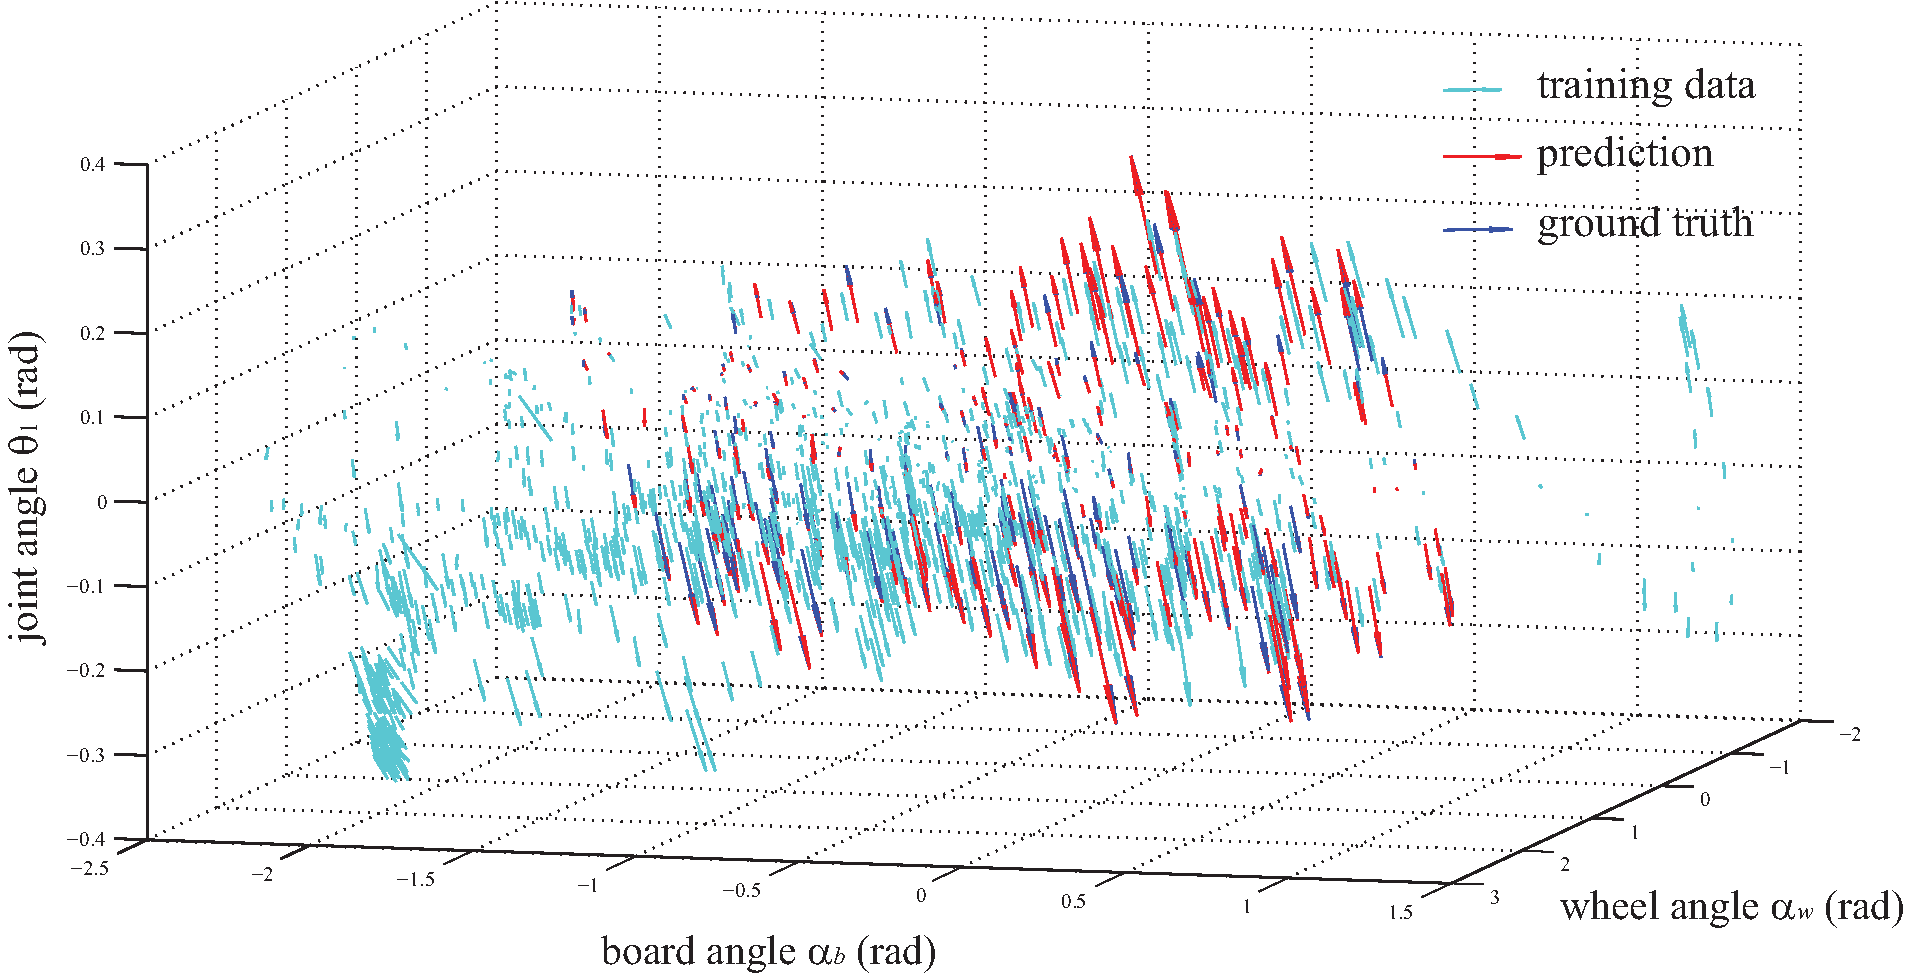
\includegraphics[width=120mm]{eps/field_00003_l03.pdf}\\
\caption{Velocity field of the learned dynamics model. Cyan: training
 data; red: prediction; blue: ground truth.}
\label{fig:learning_vector3d}
\end{center}
\end{figure*}

\subsection{Policy Search}

% basic learning results
% graphs as learning proceeds?

% learning with more model error: mass error, friction torque

We run our method for different noise levels and inertial parameter
error magnitudes to investigate the relationship between the number of
experiments required and the discrepancy between the model and hardware.
Furthermore, to test the robustness against model errors, we conducted
the same set of experiments when the inertial parameters of the Box2D
model are 20\% larger than those in the Lagrangian model.

Table~\ref{tab:learning_exp-noise} shows the average number of experiments
required to obtain a policy that can successfully balance the robot
in Box2D simulation for 5 seconds.
For reference, a 12-bit rotary encoder combined with a 50:1 gear
measures the output joint angle at a resolution of $3.1\times 10^{-5}$~rad.

The results do not show any clear relationship between the noise level
and the number of experiments required, which
implies that larger noise or error does not necessarily require more
experiments. 
Also, it is interesting that the numbers of experiments with inertial
parameter errors are generally lower than their counterparts without
errors.
We suspect that the larger inertia lowered the natural frequency of the
system, making the control easier in general.

Figure~\ref{fig:learning_cost-iteration} shows three examples of cost function
value change in Box2D simulation.
The cost generally remains flat for a few iterations and then declines
rapidly, probably when the dynamics bias model becomes accurate enough.

\begin{table}
\begin{center}
\caption{Average number of experiments required at different noise
 levels and inertial parameter errors.} \label{tab:learning_exp-noise}
\begin{tabular}{c|c|c|c|c}
\hline
Torque & Position & Velocity & 
\multicolumn{2}{c}{\# of experiments}\\\cline{4-5}
$\sigma_{\tau}^2$ & $\sigma_p^2$ & $\sigma_v^2$ & 
{\footnotesize no error} &
{\footnotesize 20\% error} \\\hline
0 & 0 & 0 & 6.4 & 2.8 \\
0.001 & 0 & 0 & 7.3 & 3.5 \\
0.01 & 0 & 0 & 9.5 & 4.8 \\
0.1 & 0 & 0 & 5.5 & 2.5 \\\hline
0.1 & $1.0\times 10^{-6}$ & $1.0\times 10^{-3}$ & 7.5 & 3.5 \\
0.1 & $2.0\times 10^{-6}$ & $2.0\times 10^{-3}$ & 4.4 & 4.4 \\
0.1 & $4.0\times 10^{-6}$ & $4.0\times 10^{-3}$ & 7.0 & 3.3 \\
0.1 & $8.0\times 10^{-6}$ & $8.0\times 10^{-3}$ & 9.6 & 5.0 \\
0.1 & $1.6\times 10^{-5}$ & $1.6\times 10^{-2}$ & 4.6 & 5.5 \\
0.1 & $3.2\times 10^{-5}$ & $3.2\times 10^{-2}$ & 4.0 & 3.5 \\
0.1 & $6.4\times 10^{-5}$ & $6.4\times 10^{-2}$ & 6.0 & 4.0 \\
0.1 & $1.28\times 10^{-4}$ & $1.28\times 10^{-1}$ & 4.0 & 3.6 \\\hline
\end{tabular}
\end{center}
\end{table}

\begin{figure}[tb]
\begin{center}
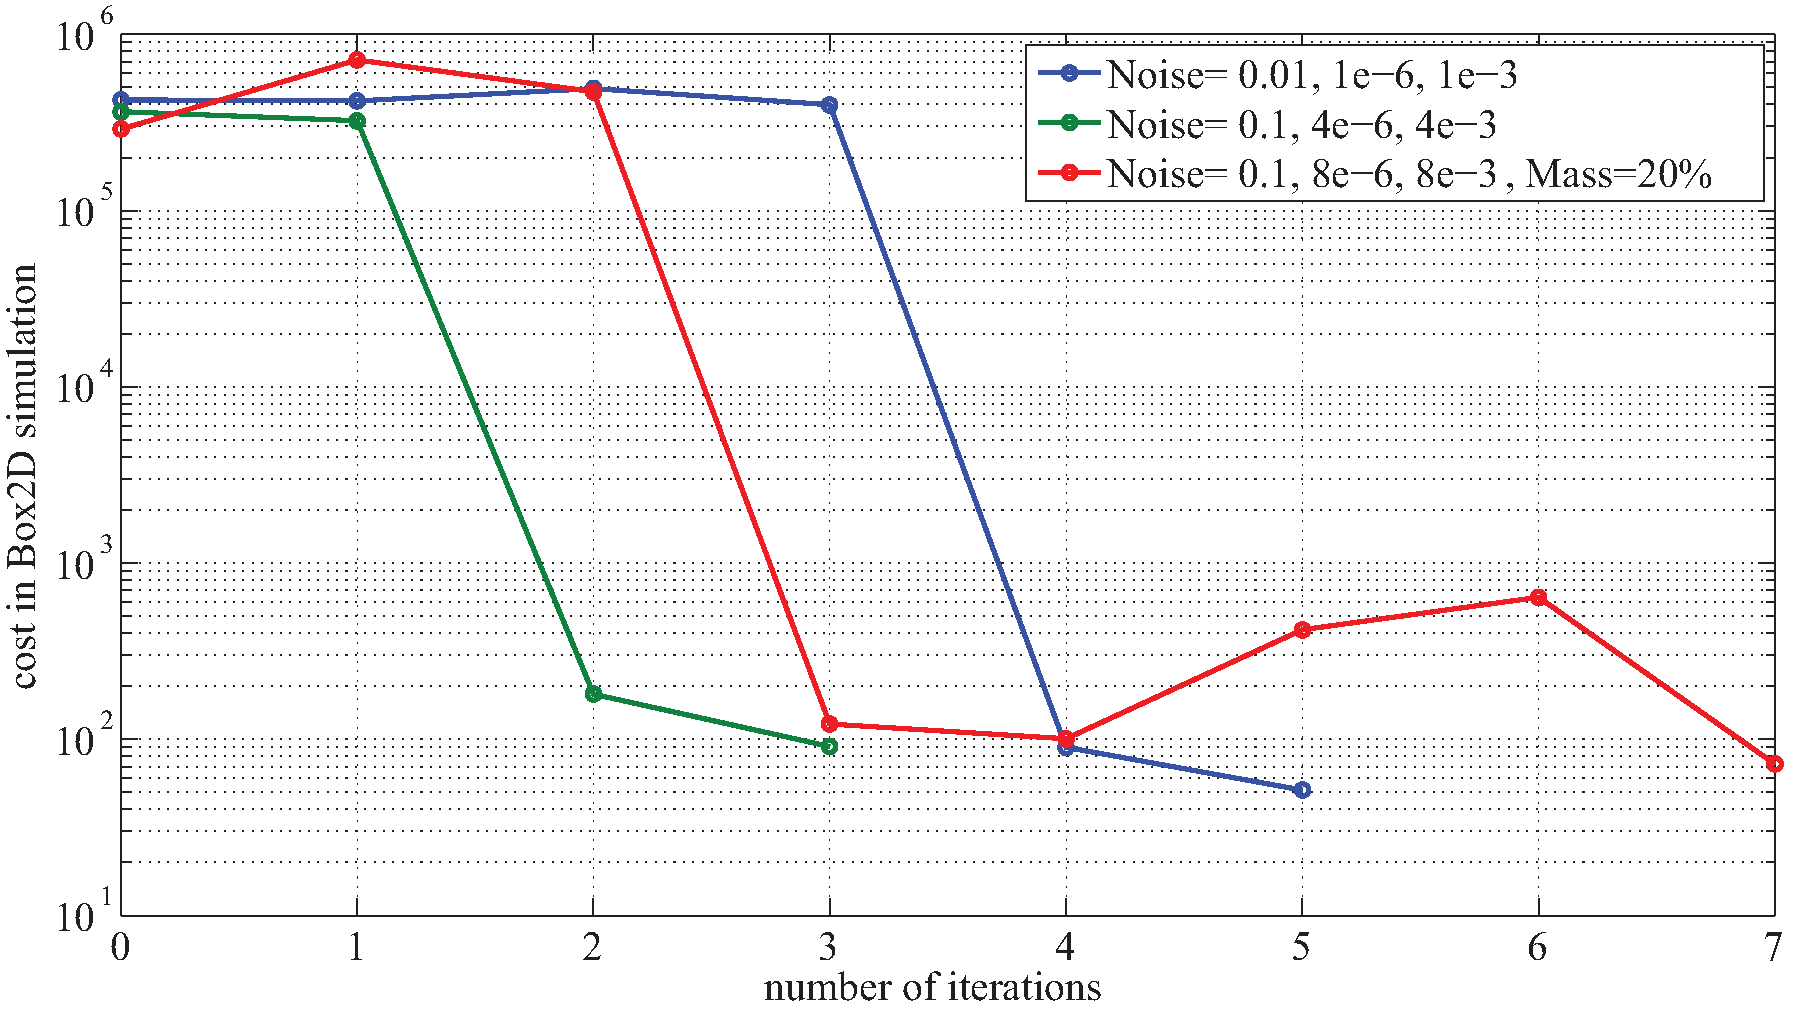
\includegraphics[width=80mm]{eps/cost_iteration.pdf}
\caption{Change of cost function value in Box2D simulations over
 iterations.}
\label{fig:learning_cost-iteration}
\end{center}
\end{figure}

\subsection{Policy Performance}

Since the Box2D simulation includes noise, simulation results vary 
even if the robot starts from the same initial state and uses the same
policy. 
We therefore compute the success rate from various initial states to
evaluate the performance of a policy.

Figure~\ref{fig:learning_success-rate} depicts the balancing success
rates starting from various wheel and board angles, using a policy
optimized with Box2D simulation without noise (a) and with noise (b).
This result clearly shows that the policy optimized in noisy environment
can successfully balance the robot from a wider range of initial states
under noisy actuator and sensors.

\begin{figure}[tb]
\begin{center}
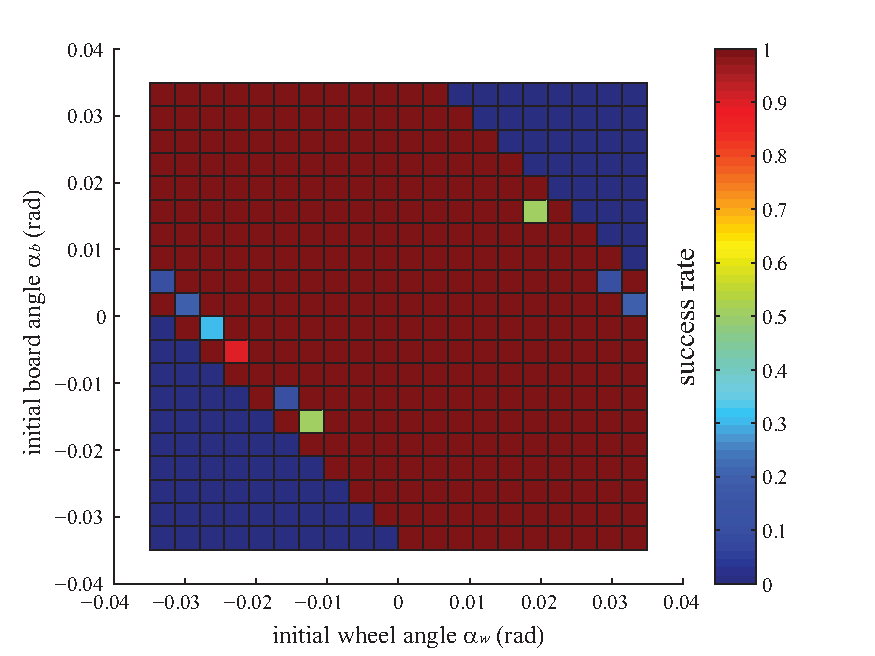
\includegraphics[width=80mm]{eps/sim_clean2_0000128.pdf}\\
(a)\\
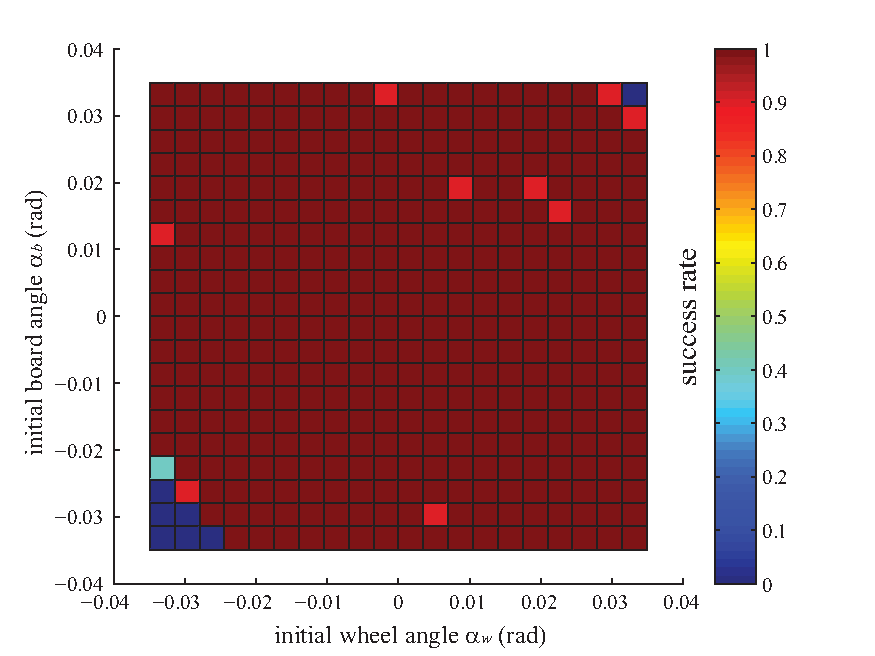
\includegraphics[width=80mm]{eps/sim_noise1_0000128.pdf}\\
(b)
\caption{Balancing success rate in Box2D simulation with noise, starting
 from various initial wheel and board angles.
(a) The policy has been optimized with Box2D simulation without noise.
(b) The policy has been optimized with Box2D simulation with noise.}
\label{fig:learning_success-rate}
\end{center}
\end{figure}

\section{Conclusion and Future Work}  \label{sec:learning_conclusion}

This paper presented a framework for model learning and policy
optimization of robots that are difficult to conduct experiments with.
The key idea is to learn the difference between a model and hardware
rather than learning the hardware dynamics from scratch.
We also employ an iterative learning process to improve the model and
policy 
This approach is particularly useful for tasks such as humanoid
balancing and locomotion where a dynamics model is necessary to obtain a
controller to collect the initial set of data.

We conducted numerical experiments through bongoboard balancing task of
a simple bipedal robot, and demonstrated that the framework can compute
a policy that successfully completes the test task with only several
hardware experiments.
The policy obtained from noisy simulation proved to have higher
balancing performance than the one obtained from clean simulation.
The number of hardware experiments did not show clear correlation with the
noise level or magnitude of inertial parameter error.

Future work besides experiments with actual hardware system includes
establishing a guideline for determining the hyper-parameters of GP and
extension to more complex robot models.
Another interesting direction would be to explore different
representation of dynamics bias instead of the additive bias considered
in this paper. 


%\bibliographystyle{plainnat}
\bibliographystyle{IEEEtran}
\bibliography{learning}

\end{document}


